% !TEX root = ../Thesis.tex
\chapter{Evaluation}
\label{c:evaluation}

This chapter is separated into two sections. The first section aims to validate and verify the implementation in terms of their
correct execution. It focuses on the core contributions, such as the lazy replicaiton algorithm as well as the freshness filter capability.
Further it ensures the correct handling of the described constraints and establishes certain test cases to identify possibile failures that can occur 
during execution as well as suitable failure handling scenarios.\\

The second part of this chapter focuses on benchmarking the implementation on the basis of the described motivational scenario itself.
This is followed by comparing the performance of several scenarios to identify how the system will behave in certain situations.
Further it will compare these executions to determine how the implementation affects the provided requirements.

Finally the performance of the individual functionalities is benchmarked and compared against slightly adjusted variations 
to give an comprehensive overview.


\section{Goal}
The evaluation has three goals: The first goal is to verify the correctness of the solution, the second goal
is identifying the impact freshness-aware aspects have on different workloads and finally the identification of suitable workloads.\\

We therefore want to verify and validate the correctness as well as the completeness of the implementation based on several characteristics.
These include the correct execution of lazy replication, the possibility to refresh statements on demand as well as correct freshness filter.

Since one of the main goals was to relax the consistency and allow parallel workloads,
we want to identify possible impacts of the replication engine on the overall performance, if freshness indeed increases the possibility
for parallel workload on the system.
Finally we want to observe if the solution allows harvesting benefits of the underlying stores to adapt to various situations
to assess the benefits of the polystore in total.\\

In general we aim to assess different situation to obtain a comprehensive insight on the introduced implementation.

%%%%%%%%%%%%%%%%%%%%%%%%%%%%%%%%%%%%%%%%%%%%%%%%%%%%%%%%%%%%%%%%%%

\section{Correctness}
\label{sec:correctness}


The correctness of the introduced solution mainly focuses on two parts. For one the replication behaviour, to verify if each lazy replication is carried out correctly,
and if not verify that reasonable counter measures are in place and apply them. This is crucial since we do not compare the footprint or the integrity of the data after 
a replication update. Rather we compare metadata of two replicasa on a high level 
(i.e. if the number of modifications and the commit timestamp after the data replication are equal on primary and secondary node). 

The second part of the validation process focuses on the retrieval of outdated nodes. Although we always have a fall back to the primary placements as described in 
section \ref{sec:fresh_select}, we still want to avoid excessive locking to parallelize requests to ultimately speed up the average response time.\\

As mentioned within the implementation chapter, several constraints (see \ref{sec:constraints}) will already be enforced with the execution itself. 
We have e.g. established a dependency between the replication strategy as well as the designated palcement state. When altering the strategy of teh object we
automatically ensure that the state is altered as well. This does not only ensure that the placements will be addressed correctly but also ensures that no data is lost.
For example it avoids that if a lazy replicated placement that still has pending replications can be switched to now receive updates eagerly.\\

Furthermore since we have to make sure that no data will be lost in general, we have established the strong dependency queue that will apply the update operation-wise in terms of the execution order.
Since we cannot avoid that stores might fail, we have ensured that failing updates will not block the replicaiton queue or will be applied in a wrong order.
Accompanied with a failure-threshols and the placement role \emph{INIFINITELY OUTDAED}, we can instruct the system to mark this placement as permanentely outdated 
avoiding further updates. 
This ensures that all statements labeled as \emph{INIFINITELY OUTDAED} will always be treated correctly.

The freshness specification in general ensures that only acceptable values are considered for the respective evaluation type to propose the correct results and translate it into
a given tolerance value.
Since freshness operations violate the ACID guarantees and we will read stale data, we ensured that these can only be executed within read-only operations, 
such that they do not override data.


Additionally, to guarantee the correctness of the implementation, several unit-tests have 
been created to ensure correct handling of data, when using freshness-awareness or replication approaches in general.
These logically include a purposely false execution of the described constrainst to ensure that they will correctly treated.\\



%%%%%%%%%%%%%%%%%%%%%%%%%%%%%%%%%%%%%%%%%%%%%%%%%%%%%%%%%%%%%%%%%%

\section{Benchmarks}

The second part of this chapter focuses on the performance impacts of the introduced solutions.
The following steps outline the procedure for benchmarking data freshness within Polypheny-DB.\\
Each evaluation step will subsequently address each required building block to provide data freshness.
Each building block is checked separetely and then put into perspective of the entire context.
These benchmark progressiviely build on top of each other and are finally summarized with a compound benchmark.\\




\subsection{Evaluation Environment}
\label{sec:env}

For all executed tests a base set of tools an functionality has been used to ensure the rerpoducibility of the benchmarks.

If not explicitly stated otherwise, the benchmarks will be executed using two underlying stores.
For these stores HSQLDB and PostgreSQL are used. While HSQLDB will run nativiely on the system, PostgreSQL is configured within a virtualized
container environment with limited resources immitating a waeker store. \\

During the evaluation only a predefined set of workloads will be used to obtain insights on various setups.
As suggested in \ref{tab:workload table} these inherently differ in terms of their focus on write- or read-operations as well the
degree of utilized freshness queries. 


\begin{table}[h]
    \centering
    \def\arraystretch{1.5}
    \begin{tabular}{V{2} l V{2} c|c|c V{2}}
    \hlineB{3}
    \textbf{Workload}        & \textbf{Read \%} & \textbf{Write \%} & \textbf{Freshness \%}  \\ \hlineB{2}
    \textbf{Write Only}      & 0                & 100               & 0                             \\ \hline
    \textbf{Mixed Workload}  & 60               & 40         & 0                             \\ \hline
    \textbf{Read Only}       & 100              & 0                 & 0                             \\ \hline
    \textbf{Freshness Only} & 100              & 0                 & 100                           \\ \hline
    \textbf{Mixed Freshness} & 60              & 40                 & 100                           \\ \hline
    \textbf{Partial Freshness} & 100              & 0                 & 100                           \\ \hlineB{2}    
    \end{tabular}
    \caption{Available Workloads}
    \label{tab:workload table}
\end{table}

Although not explictly mentioned, each test will always be pre-configured to match the required replication strategy.  

To assist the execution of the benchmarks tests a number of tools are used to standardize the procedure.

\subsubsection{Chronos}

Chronos\footnote{https://chronos-eaas.org/} is a toolkit which enables users to define, 
monitor and analyze the results of an evaluation for several database systems ~\cite{vogt_chronos_2020}.
It encompasses several tests and evaluation steps, which will be accumulated in terms of the runtime 
per target. This runtime information can then be used to compare and visualize the differences between different exectution environemnts.  



\subsubsection{OLTPBench}

For all considered tests \textit{OLTPBench}\footnote{https://github.com/oltpbenchmark/oltpbench} 
has been used. This benchmarking framework bundles several workload classes and 
encompasses multiple benchmarking tools to seamlessly provide benchmarking for various DBMS \cite{oltp_2013}.\\
To get a more in-depth view how the implementation affected the overall performance, all following tests have been executed 
using \textit{YCSB}\footnote{https://github.com/brianfrankcooper/YCSB}.
YCSB not only offers a fundamental correctness test but additionally simulates workload on a single table to obtain essential performance baselines ~\cite{ycsb_2010}.
These can be used to retrieve performance metrics and obtain indications regarding correct statement execution and query handling.\\


%%%%%%%%%%%%%%%%%%%%%%%%%%%%%%%%%%%%%%%%%%%%%%
%%%%%%%%%%%%%%%%%%%%%%%%%%%%%%%%%%%%%%%%%%%%%%

\subsection{Results}
\label{sec:results}
In this section we will present the results of the performance evaluation.

If not stated otherwise the generated tables within the benchmarks will contain 100000 entries and will be executed using
50 parallel client threads, using YCSB and the workloads as defined in table \ref{tab:workload table}.
During the evaluation it will only be referred to the respective workload names.

           
\todoMissing{Story - konzept nicht Abstrakt und warum mit Polystore gut - mit Motivation verknüpfen}

\subsubsection{Overhead} 
Polystore systems and specifically Polypheny-DB uniformly collect all incoming requests, process them and then
route the resulting queries to the designated stores, where they will be finally executed. 
However, due to this centralized processing, addtional introduced overhead within this layer will directly impact the performance of the system.
Although, Polypheny-DB aims to provide cost- and workload-aware self-adaptiveness, to provide the best possible query results,
its internal processing is executed on top of the actual execution of the underlying store.
This can have a crucial impact on the entire throughput of the system.\\
Hence we used Chronos, a benchmarking tool that allows us to define several evaluation steps per storage engine,
to measure the overhead. For this evaluation the introduced implementation is compared against the current state of Polypheny-DB.\\

As depicted in Figure \ref{fig:overhead}, the results indeed show that the implementation introduced a little overhead for single store operations.
However with multiple stores the actual average execution time was indeed slightly reduced. Although, single store executions should not be entirely neglected
they do not form the main pursuit of polystore systems, which are more suitably visualized by the multistore runtime.



\begin{figure}[t] 
    \centering 
    \begin{tikzpicture}
        \begin{axis}[
            width  = 0.85*\textwidth,
            height = 7cm,
            x=120pt,
            major x tick style = transparent,
            ybar=.2cm,
            bar width=30pt,
            ymajorgrids = true,
            ylabel = {Runtime (ms)},
            xlabel = {Number of Stores},
            symbolic x coords={1,2},
            xtick = data,
            scaled y ticks = false,
            enlarge x limits=0.40,
            ymin=0,
            major tick style={thick},
            legend pos=outer north east,
            legend cell align=left,
        ]
            \addplot[style={bblue,fill =bblue,mark=none}]
                coordinates {(1, 1454546 ) (2,1712337)};

            \addplot[style={rred,fill=rred,mark=none}]
                coordinates {(1, 1569320) (2,1629462) };

            \legend{Old,New}
        \end{axis}
    \end{tikzpicture}
\caption{Overhead Comparison of Old vs. New Implemation.}
\label{fig:overhead}
\end{figure}



%%%%%%%%%%%%%%%%%%%%%%%%%%%%%%%%%%%%%%%%%%%%%%%%%%%%%%%%%%%%%%%%%%

\subsubsection{Locking-Mechanism} 

As described in Section \ref{sec:strategy}, one of the prerequisites to establish multiple refresh strategies and hence lazy replication,  
was the refactoring of the locking mechanism. Although, not completely reworked, the locking-module of Polyphenys SS2PL 
poses as a core component of the system. It therefore  impacts correct serializability treatement and is and inherent driver of 
the concurrency which directly influences the overall performance of the system.\\
For the evaluation again the current state of Polypheny-DB is compared against this implementation.
Since the locking module was changed from a table-wise locking towards a partition-wise locking we will validate the impact on the basis of 
a single table using YCSB. 
The evaluation was executed with gradually increasing numbers of partitions, which are placed on one store or distributed across $n$-Stores 
for $n$ partitions to observe any changes on the locking and therefore the throughput.\\
To get a general overview of the impact, the benchmark was executed using a mixed workload using HSQLDB only.\\


%%%%%%%

\begin{figure}[t]
    \centering
    \begin{subfigure}{.5\textwidth}
      \centering
      \begin{tikzpicture}
        \begin{axis}[
            width  = 0.9*\textwidth,
            ymajorgrids = true,
            ylabel = {Throughput (requests/s)},
            xlabel = {Number of Partitions ($n$)},
            symbolic x coords={2,4,8},
            xtick = data,
            scaled y ticks = false,
            enlarge x limits=0.40,
            ymin=60,
            ymax=140,
            legend style={
                    at={(1,1.05)},
                    anchor=south east,
                    column sep=1ex
            },
            legend cell align=left,
            smooth
        ]
            \addplot[style={bblue,mark=*}]
                coordinates {(2, 82.66787244) (4,110.0694971) (8,124.4930924)};

            \addplot[style={rred,mark=x}]
                coordinates {(2, 90.32423012) (4,85.38185074) (8,69.04305019)};

            \legend{Single Store,$n$ Stores}
        \end{axis}
    \end{tikzpicture}
      \caption{Old Locking}
      \label{fig:oldlock}
    \end{subfigure}%
    \begin{subfigure}{.5\textwidth}
      \centering
      \begin{tikzpicture}
        \begin{axis}[
            width  = 0.9*\textwidth,
            ymajorgrids = true,
            ylabel = {Throughput (requests/s)},
            xlabel = {Number of Partitions ($n$)},
            symbolic x coords={2,4,8},
            xtick = data,
            scaled y ticks = false,
            enlarge x limits=0.40,
            ymin=60,
            ymax=140,
            major tick style={thick},
            legend style={
                    at={(1,1.05)},
                    anchor=south east,
                    column sep=1ex
            },
            legend cell align=left,
            smooth
        ]
            \addplot[style={bblue,mark=square*}]
                coordinates {(2, 83.56813262) (4,118.5016919) (8,136.0429577)};

            \addplot[style={rred,mark=diamond*}]
                coordinates {(2, 75.87686445) (4,90.53951027) (8,68.78432784)};

            \legend{Single Store,$n$ Stores}
        \end{axis}
    \end{tikzpicture}
      \caption{New Locking}
      \label{fig:newlock}
    \end{subfigure}
    \begin{subfigure}{.7\textwidth}
        \centering
        \begin{tikzpicture}
            \begin{axis}[
                width  = 0.7*\textwidth,
                ymajorgrids = true,
                ylabel = {Throughput (requests/s)},
                xlabel = {Number of Partitions ($n$)},
                symbolic x coords={2,4,8},
                xtick = data,
                scaled y ticks = false,
                enlarge x limits=0.40,
                minor y tick num=3,
                ymin=60,
                ymax=140,
                major tick style={very thick},
                legend pos=outer north east,
                legend cell align=left,
                smooth
            ]
                \addplot[style={bblue,mark=*}]
                    coordinates {(2, 82.66787244) (4,110.0694971) (8,124.4930924)};
    
                \addplot[style={rred,mark=square*}]
                    coordinates {(2, 83.56813262) (4,118.5016919) (8,136.0429577)};
    
                \legend{Old,New}
            \end{axis}
        \end{tikzpicture}
        \caption{Old vs. New Locking}
        \label{fig:oldandnewlock}
      \end{subfigure}
    \caption{Impact of Locking on the Overall Throughput per Second.}
    \label{fig:lock_comp}
\end{figure}


As visualized in Figure \ref{fig:oldlock} and \ref{fig:newlock}, for both cases the overall situation is quite similiar.
While the distribution of the partitions across several stores gets gradually worse, the single store performance actually improves the more partitions are added to the table.
This behaviour is essentially caused by Polyphenys need to join and union several stores together, when querying multiple partitions across several stores.
Since more stores need to be connected and considered, it is a rather costly approach and as stated before gets increasingly harder the more stores are involved.\\

Because the single store variations prove to be more reliable, they are summarized in \ref{fig:oldandnewlock}.
We can observe that the new locking mechanism indeed proves to be slightly better in terms of the possible throughput.
Furthermore it shows that again with a growing number of stores, the gap between the old and new locking extends even more, validating the benefits of the new locking mechanisms.




%%%%%%%%%%%%%%%%%%%%%%%%%%%%%%%%%%%%%%%%%%%%%%%%%%%%%%%%%%%%%%%%%%


\subsubsection{Baseline Identification} 

%%%%%%%%%%%%%%%%%%%%%%%%%%%%%%%%%%%%%%%%%
% Single Store performance of HSQL and PSQL
%%%%%%%%%%%%%%%%%%%%%%%%%%%%%%%%%%%%%%%%%

Since the Lazy Replication algorithm is not only fundamental to generate multiple versions to be used within freshness-awareness
but also a core functionality how data is propagated throughout the system. 
Hence, along with the newly introduced replication strategies, and \emph{Change Data Collection} it will have a major impact on the overall perfromance of the system.
Since the replication solely focuses on replicating captured changes, the next benchmarks will be consequently executed using only DML-operations without any reads.\\

\begin{figure}[t] 
    \centering 
    \begin{tikzpicture}
        \begin{axis}[
            width  = 0.85*\textwidth,
            height = 7cm,
            x=80pt,
            major x tick style = transparent,
            ybar=.2cm,
            bar width=30pt,
            ymajorgrids = true,
            ylabel = {Avg. Response Time (ms)},
            xlabel = {Stores},
            symbolic x coords={HSQLDB,PostgreSQL},
            xtick = data,
            scaled y ticks = false,
            enlarge x limits=0.50,
            minor y tick num=4,
            ymin=0,
            ymax=3000,
            major tick style={thick},
            legend pos=outer north east,
            legend cell align=left,
        ]
            \addplot[style={bblue,fill=bblue,mark=none}]
                coordinates {(HSQLDB, 2210 ) (PostgreSQL,2700)};

        \end{axis}
    \end{tikzpicture}
    \caption{Single Write Time Comparison. PostgreSQL vs. Single HSQLDB.}
    \label{fig:singlepsqlhsql}
\end{figure}

As stated in the evaluation environment \ref{sec:env}, these benchmarks will be mainly executed with an embedded version of HSQLDB and PostgreSQL running within a virtualized 
container environment. To have a general base line for comparison Figure \ref{fig:singlepsqlhsql} presents a single store execution, comparing theses two stores against each other.
As motivated in the beginning, it is crucil for a system to utilize the key benefits of each store. For our scenario this is important to determine which 
store configuration is more suitable to be used as an eagerly replicated primary placement, due to its lower latency and better reponse time.\\
This illustreated comparison clearly shows that Due to its limited resources the PostgreSQL store cannot directly compete with this HSQLDB configuration.
This provides us with the intuitive decission to use HSQLDB for the priamry transactions.




%%%%%%%%%%%%%%%%%%%%%%%%%%%%%%%%%%%%%%%%%%%%%%%%%%%%%%%%%%%%%%%%%%




\subsubsection{Lazy Replication} 

%%%%%%%%%%%%%%%%%%%%%%%%%%%%%%%%%%%%%%%%%
% Terminal 1 vs. Terminal 50
%%%%%%%%%%%%%%%%%%%%%%%%%%%%%%%%%%%%%%%%%

As previously stated, the replication strategies will impact the processing capability of the system immensly.
A placement with a configured lazy replication strategy automatically enables the system, to start tracking changes for this entity, impacting the duration of a query.
Therfore we want to compare how each store handles the replication differently. Consequently we want to benchmark and compare two equal placements that are eagerly replicated
against the same two stores but one configured as \emph{lazy}.\\

To extend the baseline discovered before, we again want to demonstrate the behaviour a purely sequential environment with only one client has, 
against a parallel environment with 50 clients.\\
Figure \ref{fig:terminal} shows the evaluation across two stores, providing the possible throughput per second. Which is given as the number of modifications that can be 
applied to the system per second. As before HSQLDB obviously achieves better results then PostgreSQL. However what is surprising is that disregarding the store,
the eagerly replicated configuration performs much better in all tests which is not apparent when only considering \ref{fig:terminal50}.
Considering that the collection of changes within a llazy setup, indeed imposes additional costs on the processing time, such deviations are expected.

\begin{figure}[t]
    \centering
    \begin{subfigure}{.5\textwidth}
      \centering
      \begin{tikzpicture}
        \begin{axis}[
            width  = 0.7*\textwidth,
            x=80pt,
            major x tick style = transparent,
            ybar=.2cm,
            bar width=20pt,
            ymajorgrids = true,
            ylabel = {Throughput (requests/s)},
            xlabel = {Replication Strategy},
            symbolic x coords={Eager,Lazy},
            xtick = data,
            scaled y ticks = false,
            enlarge x limits=0.40,
            ymin=0,
            ymax=30,
            major tick style={thick},
            legend style={
                    at={(1,1.05)},
                    anchor=south east,
                    column sep=1ex
            },
            legend cell align=left,
        ]
            \addplot[style={bblue,fill =bblue,mark=none}]
                coordinates {(Eager, 26.15944582) (Lazy,19.0566423)};

            \addplot[style={rred,fill=rred,mark=none}]
                coordinates {(Eager, 16.9502111) (Lazy,11.78997423) };

            \legend{HSQLDB,PostgreSQL}
        \end{axis}
    \end{tikzpicture}
      \caption{One process}
      \label{fig:terminal1}
    \end{subfigure}%
    \begin{subfigure}{.5\textwidth}
      \centering
      \begin{tikzpicture}
        \begin{axis}[
            width  = 0.7*\textwidth,
            x=80pt,
            major x tick style = transparent,
            ybar=.2cm,
            bar width=20pt,
            ymajorgrids = true,
            ylabel = {Throughput (requests/s)},
            xlabel = {Replication Strategy},
            symbolic x coords={Eager,Lazy},
            xtick = data,
            scaled y ticks = false,
            enlarge x limits=0.40,
            ymin=0,
            ymax=30,
            major tick style={thick},
            legend style={
                    at={(1,1.05)},
                    anchor=south east,
                    column sep=1ex
            },
            legend cell align=left,
        ]
            \addplot[style={bblue,fill =bblue,mark=none}]
                coordinates {(Eager, 19.08643067 ) (Lazy,14.62659111)};

            \addplot[style={rred,fill=rred,mark=none}]
                coordinates {(Eager, 15.52999761) (Lazy,11.86666016) };
                

                \legend{HSQLDB,PostgreSQL}
        \end{axis}
    \end{tikzpicture}
      \caption{50 processes}
      \label{fig:terminal50}
    \end{subfigure}
    \caption{Concurrency Comparison}
    \label{fig:terminal}
\end{figure}


Admittingly an enitity that is composed of only similiar or equal stores, will not be beneficial for a polystore system, to allow different workloads.
Therefore the follwoing benchmarks will concentrate on a mixed setup with interleaved stores. Furthermore these tests will be executed with 50 parallel clients to repoduce a 
conventional environment. 

%%%%%%%%%%%%%%%%%%%%%%%%%%%%%%%%%%%%%%%%%%%%%%%%%%%%%%%%%%%%%%%%%%

%%%%%%%%%%%%%%%%%%%%%%%%%%%%%%%%%%%%%%%%%
% HSQL and PSQL vs. Eager
%%%%%%%%%%%%%%%%%%%%%%%%%%%%%%%%%%%%%%%%%

Now focussing on a mixed setup of two stores containing PostgreSQL as well as HSQLDB for one entity.
Nativiely for a polystore environment we want to identify which setup of underlying stores will produce better results, hence is suitable for which situation.
Consequently we want to observe how the order of the stores imapcts the response time per benchmark.\\
Again to have a foundation to compare our changes to we will compare the configurations if both stores are defined as eager and Further
respectiviely define each store as lazy as well.\\
Ultimately \ref{fig:psqlhsqlresponse} shows that regarding the lazy approaches, we again see the common behaviour that HSQLDB performs a little better as an eagerly replicated
store compared to PostgreSQL.

\begin{figure}[t] 
    \centering 
    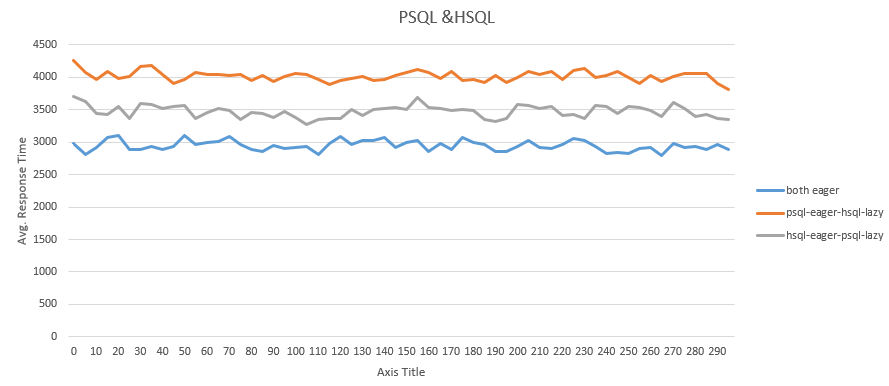
\includegraphics[width=0.7\textwidth]{Figures/PSQ_HSQL_DML_only.PNG}
    \caption{DML only - Avg. Latency comparsion PostgreSQL vs. HSQLDB. With switching Roles}
    \label{fig:psqlhsqlresponse}
\end{figure}

Additionally the Figure in \ref{fig:overall_comp} puts the average latency in perspective to the execution times described before.
As one can observe the eager replications again pefrom the best while the PostgreSQL variation posing a eager perfroms the worst.
This not only allows to compare the different setups but again aids us to choose suitable combinations for our designated tasks.\\



\begin{figure}[t] 
    \centering 
    \begin{tikzpicture}
        \begin{axis}[
            width  = 0.7*\textwidth,
            x=80pt,
            major x tick style = transparent,
            ybar=.2cm,
            bar width=20pt,
            ymajorgrids = true,
            ylabel = {Avg. Response Time (ms)},
            xlabel = {Store Compositions},
            symbolic x coords={1},
            xtick = data,
            xticklabels={},
            scaled y ticks = false,
            enlarge x limits=0.40,
            ymin=0,
            ymax=4500,
            minor y tick num=4,
            major tick style={thick},
            legend pos=outer north east,
            legend cell align=left,
        ]
            \addplot[style={bblue,fill =bblue,mark=none}]
                coordinates {(1, 2598.875133)};    
            
            \addplot[style={rred,fill=rred,mark=none}]
                coordinates {(1, 3194.893767)};    

            \addplot[style={ggreen,fill =ggreen,mark=none}]
                coordinates {(1, 2948.031083)};

            \addplot[style={ppurple,fill=ppurple,mark=none}]
                coordinates {(1, 4018.661833)};

            \addplot[style={orange,fill =orange,mark=none}]
                coordinates {(1, 3475.416683)};

            \legend{ 
                HSQLDB x2 (Eager),
                PostgreSQL x2 (Eager),
                PostgreSQL (Eager) - HSQLDB (Eager),
                PostgreSQL (Eager) - HSQLDB (Lazy), 
                HSQLDB(Eager) - PostgreSQL(Lazy),
                }
        \end{axis}
    \end{tikzpicture}
    \caption{DML onlyAvg. Response Time Comparison of 2 store sizes and swithcing Roles}
    \label{fig:overall_comp}
\end{figure}


%%%%%%%%%%%%%%%%%%%%%%%%%%%%%%%%%%%%%%%%%
% Store Scale 2 vs. 4 HSQL and PSQL
%%%%%%%%%%%%%%%%%%%%%%%%%%%%%%%%%%%%%%%%%

However, the presented possibilities so far only considered the execution on two stores. Therefore, \ref{fig:24storecomp} aims
to compare the execution on two and four stores to identify any deviations the lazy replicaiton algorithm has. 
Again this is done in an interleaved fashion, switching the role of lazy and eager strategy between the participating stores.
During theses tests only one is eagerly replicated the remaining are all configured as lazy placements. Eagerly and lazily replicated stores
in this scenario are inherently defined to be different stores.\\
The graphs indicate that although they differ in terms of average response times, the gap between both configurations is comparably equal.
In both cases the execution with the eagerly replicated HSQLDB is roughly 500ms faster in terms of the average response time.\\


\begin{figure}[t]
    \centering
    \begin{subfigure}{.5\textwidth}
      \centering
      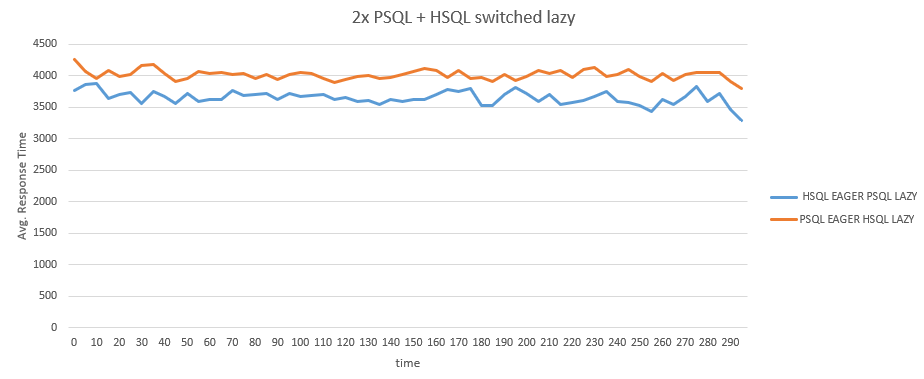
\includegraphics[width=.9\linewidth]{psql_hsql_switched_lazy.PNG}
      \caption{Comparison of 2 Stores HSQLDB and PostgreSQL. Switching Roles.}
      \label{fig:2store}
    \end{subfigure}%
    \begin{subfigure}{.5\textwidth}
      \centering
      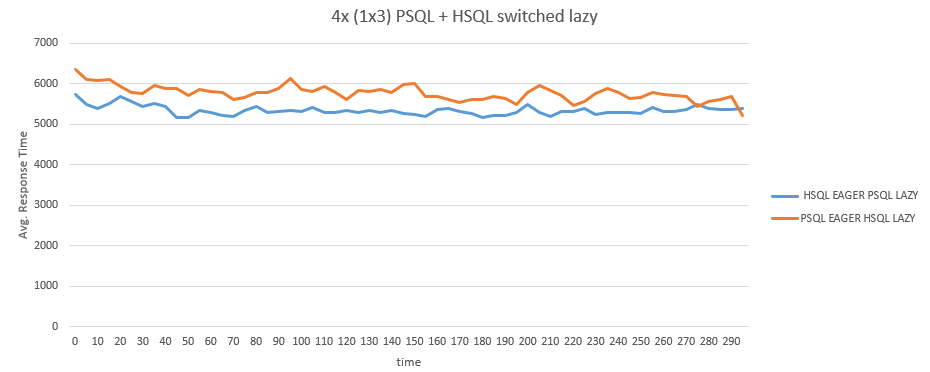
\includegraphics[width=.9\linewidth]{Figures/4psql_hsql_switched_lazy.PNG}
      \caption{Comparison of 4 Stores HSQLDB and PostgreSQL. Switching Roles.}
      \label{fig:4store}
    \end{subfigure}
    \caption{Comparison of different store sizes and swithcing Roles}
    \label{fig:24storecomp}
\end{figure}


\begin{figure}[t] 
    \centering 
    \begin{tikzpicture}
        \begin{axis}[
            width  = 0.9*\textwidth,
            height = 7cm,
            x=120pt,
            major x tick style = transparent,
            ybar=.2cm,
            bar width=30pt,
            ymajorgrids = true,
            ylabel = {Avg. Response Time (ms)},
            xlabel = {Number of Stores},
            symbolic x coords={2,4},
            xtick = data,
            scaled y ticks = false,
            enlarge x limits=0.40,
            ymin=0,
            ymax=6000,
            minor y tick num=4,
            major tick style={thick},
            legend style={
                    at={(1,1.05)},
                    anchor=south east,
                    column sep=1ex
            },
            legend cell align=left,
        ]
            \addplot[style={bblue,fill =bblue,mark=none}]
                coordinates {(2, 3653.642433) (4,5346.252567 )};

            \addplot[style={rred,fill=rred,mark=none}]
                coordinates {(2, 4018.661833) (4,5771.588467) };

            \legend{HSQLDB(Eager) - PostgreSQL(Lazy),
                PostgreSQL (Eager) - HSQLDB (Lazy) 
            }
        \end{axis}
    \end{tikzpicture}
    \caption{Avg. Response Time Comparison of different store sizes and swithcing Roles}
    \label{fig:24storecomp_avg}
\end{figure}


As summarized and visualized more densely in Figure \ref{fig:24storecomp_avg},
its rather counter intuitive that the configurations in \ref{fig:24storecomp} (a) and (b) deviate at all. 
In general they both only contain one primary placement that is even targeted for the primary transaction.
All other stores will be updated asynchronously and therefore not directly involved.
However, as described before, the primary transaction is also responsible for capturing, as well as queing the changes to be replicated asynchronously.
While the procedure is always executed equally, the second approach with four stores, has more replication targets that require the change. 
Since the generation of replication objects as well as the queueing are all still done during the commit of the primary transaction, the observed
deviations are reasonable.\\


%%%%%%%%%%%%%%%%%%%%%%%%%%%%%%%%%%%%%%%%%
% Store Scale 2-8
%%%%%%%%%%%%%%%%%%%%%%%%%%%%%%%%%%%%%%%%%
Based on this observation we specifically wanted to compare how a growth in stores will impact this deviation and how it compares against its eager counterpart. 
To have a more uniform result this test will be executed only HSQLDB stores, to have a stable foundation for comparison
without a second store that could interfere with the final result.\\
In this evaluation \ref{fig:stores_comp} illustrates, the average response time of two to eight stores, where one store is eagerly replicated and the rest
is configured as lazy.


\begin{figure}[t] 
    \centering 
    \centering
        \begin{tikzpicture}
            \begin{axis}[
                width  = 0.7*\textwidth,
                height = 7cm,
                ymajorgrids = true,
                ylabel = {Avg. Response Time (ms)},
                xlabel = {Number of Stores},
                symbolic x coords={2,4,8},
                xtick = data,
                scaled y ticks = false,
                enlarge x limits=0.40,
                minor y tick num=3,
                ymin=0,
                ymax=6000,
                major tick style={very thick},
                legend pos=outer north east,
                legend cell align=left,
                smooth
            ]
                \addplot[style={bblue,mark=*}]
                    coordinates {(2, 2598.875133) (4,3441.368233) (8,4911.982467)};
    
                \addplot[style={rred,mark=x}]
                    coordinates {(2, 3492.3136) (4,3943.186767) (8,5532.865083)};
    
                \legend{Eager,Lazy}
            \end{axis}
        \end{tikzpicture}
    \caption{Replication Strategy Comparison with Increased Stores}
    \label{fig:stores_comp}
\end{figure}

This indicates that although the repsonse time increases, it does so in a stable manner. As compared with its eager approach we can see that it evolves roughly towards teh same direction plus
previously observed offset, providing a good scalability.

\subsubsection{Queue Replication}

%%%%%%%%%%%%%%%%%%%%%%%%%%%%%%%%%%%%%%%%%
% Single operation comparison
%%%%%%%%%%%%%%%%%%%%%%%%%%%%%%%%%%%%%%%%%

As presented during the implementation and now ellaborated and suggested multiple times during evaluation, 
the capture of modifications to be propagated to the secondary placements, introduces some overhead. Although some overhead
is reasonable due to the additional processing steps, the response times differ 
especially when compared to regular eagerly replicated scenarios. This directly impacts the overall performance,
resulting in generally higher response times for lazy replication scenarios.
Therefore we want to identify for a single write-operation what actually influences these runtime deviations.


\begin{figure}[t] 
    \centering 
    \begin{tikzpicture}
        \begin{axis}[
            width  = 0.8*\textwidth,
            height=6cm,
            ybar stacked,
            x=80pt,
            major x tick style = transparent,
            bar width=30pt,
            ymajorgrids = true,
            ylabel = {Execution Time (ms)},
            xlabel = {Replication Statements},
            symbolic x coords={Eager, Lazy},
            xtick = data,
            scaled y ticks = false,
            enlarge x limits=0.40,
            ymin=0,
            ymax=70,
            minor y tick num=4,
            major tick style={thick},
            legend pos=outer north east,
            legend cell align=left,
        ]
            \addplot+[ybar][style={bblue,fill =bblue,mark=none}]
                coordinates {(Eager, 21) (Lazy, 18)};

            \addplot+[ybar][style={rred,fill=rred,mark=none}]
                coordinates {(Eager, 0) (Lazy, 16)};

            \addplot+[ybar][style={ppurple,fill =ppurple,mark=none}]
                coordinates {(Eager, 0) (Lazy, 28)};

            \legend{ 
                Base Execution,
                Capture Queue,
                Replication,
                }
        \end{axis}
    \end{tikzpicture}
    \caption{Execution-Time comparision of a decompossed  single write-operation with and without data active data capture }
    \label{fig:write_decomposition}
\end{figure}



The comparison in Figure \ref{fig:write_decomposition} analyzes the execution time of two independent write operations, respectiviely executed on two equal stores.
One configuration is a simple eager replicated entity on two stores without any replication, the other one is an operation that needs to capture 
the modification within the global replication queue.\\
Since the lazy approach only needs to involve one store for processing, the baseline of the lazy approach is indeed slightly faster than its eager counterpart.
However, considering that at commit time this approach also needs to extract the captured change, convert it into a replication object and ultimately queue 
it for the remaining store, the actual execution deviates quite heavily. With the queue time being almost equal to its the base execution time.\\
However, since the capture part is only executed once at commit time of a transaction it drastically impacts the performance 
of one single operation.
As we have seen before, this introduced capture gap remains quite stable even with additional targets or capture objects to transform.
Therefore the queueing process negativiely impacts the efficiency for transactions containing only one or few operations.
In contrast it gets neglected further the more operations are actually executed within one transaction.\\
Additionally, although not directly considered to be part of the execution time, is the convergence window. As mentioned before, as soon
as a replication worker will have free resources it will replicate the pending object from the queue onto the secondary store.
As we can see the replication duration actually takes a little bit longer than the actual execution. This is caused by the introduced
validation constraints for each worker to assess the queue and reconstruct each opeartion individually. 
However since the replication is done operation-wise the replication time is considered to be fixed per operation.
Therfore the entire bar immitates the time it takes for one operation to be executed and replicated across all participating store, 
considering the aforementioned constraints of the queue time.
Since the eagerly replicated approach is executed within one single transaction targeting both underlying stores, the entity is 
considered to be immediately consistent and will not need to converge. 






%%%%%%%%%%%%%%%%%%%%%%%%%%%%%%%%%%%%%%%%%%%%%%%%%%%%%%%%%%%%%%%%%%


\subsubsection{Replica Convergence} 

\todoMissing{Story-concrete example}



\begin{figure}[t] 
    \centering 
    \begin{tikzpicture}
        \begin{axis}[
            width  = 0.9*\textwidth,
            height = 7cm,
            x=120pt,
            major x tick style = transparent,
            ybar=.2cm,
            bar width=30pt,
            ymajorgrids = true,
            ylabel = {Execution Time (sec)},
            xlabel = {Number of Stores},
            symbolic x coords={2,4},
            xtick = data,
            scaled y ticks = false,
            enlarge x limits=0.40,
            ymin=0,
            ymax=45,
            minor y tick num=4,
            major tick style={thick},
            legend style={
                    at={(1,1.05)},
                    anchor=south east,
                    column sep=1ex
            },
            legend cell align=left,
        ]
            \addplot[style={bblue,fill =bblue,mark=none}]
                coordinates {(2, 33.4120) (4,39.18 )};

            \addplot[style={rred,fill=rred,mark=none}]
                coordinates {(2, 30.322) (4,36.9) };

            \legend{HSQLDB(Eager) - PostgreSQL(Lazy),
                PostgreSQL (Eager) - HSQLDB (Lazy) 
            }
        \end{axis}
    \end{tikzpicture}
    \caption{Comparison of Convergence Time on different Store Constellations.}
    \label{fig:store_comparision}
\end{figure}

As we have seen before the versions can deviate quite heavily during a mixed workload. 
Furthermore we have already identified that configuring the faster perfoming store to be replicate eagerly, proofs that this will positiviely impact 
the availability due to its lower repsonse time of the inital transaction.
However as important as the throughput of initial transaction might be, choosing the faster node to be eagerly replicated intuitively leaves the slower node
to apply the updates asynchronously. 
However, because it highly depends on the requirements which configuration to choose, we also want to establish a setup that focuses on reaching
a consistent state without using an eager-only replication setup.



Therefore we want to observe the actual replication time until two stores reach an equilibrium in terms of their received updates.\\
The plot in \ref{fig:store_comparision} visualizes the comparison based on a different number of stores.

Due to the fact that HSQLDB was before identifed as the store with the better throughput, 
it also generally manages to converge faster if configured to be the secondary store. 
Since HSQLDB in our scenario is able to replicate the operations faster than the primary transaction can queue new events,
it does not only converge faster but has a lower execution time in general.\\
Therefore we have established that with our introduced algorithm, indeed
the better performing store is also more suitable when we want to reach consistency faster, hence providing a smaller convergence time.\\




Although that the convergence time is not essentially impacted by the executing store, but also by the number of designated stores that shall asynchronously 
receive the operation. 
Further we want to identify how the queue behaves if the secondary system is generally slower and therefore not able to replicate 
the pending changes as fast as new ones are added to the queue.


\begin{figure}[t]
    \centering
    \begin{subfigure}{.5\textwidth}
      \centering
      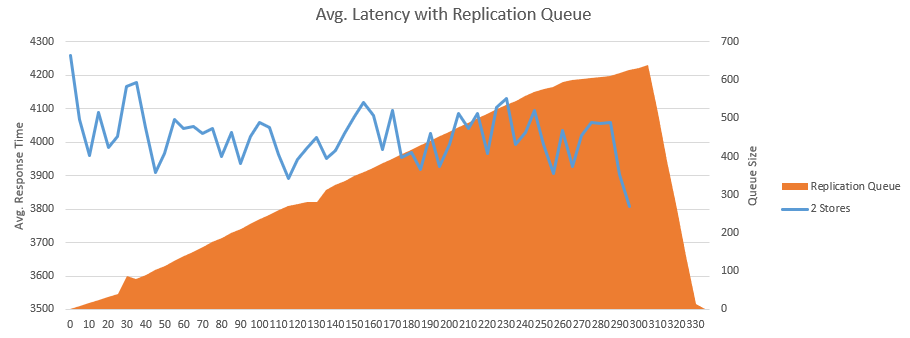
\includegraphics[width=.9\linewidth]{Figures/2latency_queue.PNG}
      \caption{2 Stores}
      \label{fig:converge_2}
    \end{subfigure}%
    \begin{subfigure}{.5\textwidth}
      \centering
      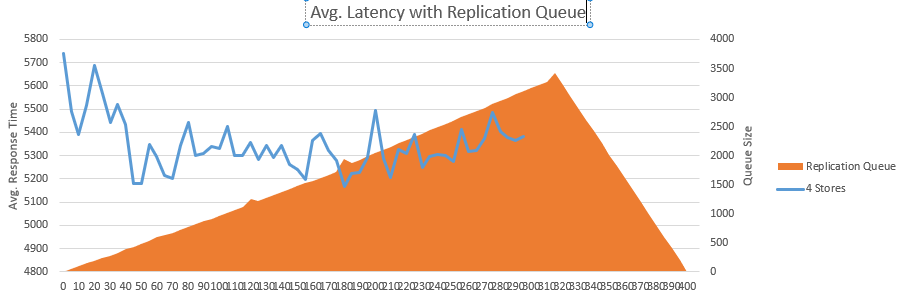
\includegraphics[width=.9\linewidth]{Figures/4latence_queue.PNG}
      \caption{4 Stores}
      \label{fig:converge_4}
    \end{subfigure}
    \caption{Execution Time and Replication Convergence}
    \label{fig:converge_24}
\end{figure}


Figure \ref{fig:converge_24} visualizes the expansion- as well as the shrinking-phase of the replication queue
and puts it into perspective along with the actual test execution. During theses tests one worker continuously processed the queue and replicated 
the changes operation-wise. As illustrated in both cases the worker is not really able to apply the changes faster than they are coming in.
The breakeven point is reached as soon as the test execution has finished. For both configurations the algorithm can now quickly propagate all pending
changes.\\

\begin{figure}[t] 
    \centering 
    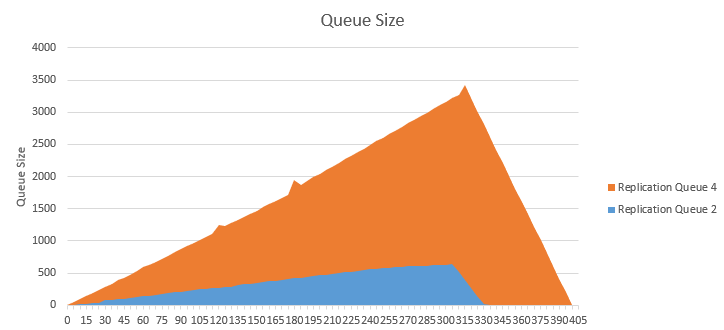
\includegraphics[width=0.7\textwidth]{Figures/queuesize24.PNG}
    \caption{Replication Queue Convergence}
    \label{fig:converge24}
\end{figure}


Because captured change operations are transformed $1-n$ for $n$ lazy replicated stores, the size of the queues is essentially influenced by the number of replicas that
require the change as summarized in Figure \ref{fig:converge24}. This directly influences the earlier described convergence time of our system.







%%%%%%%%%%%%%%%%%%%%%%%%%%%%%%%%%%%%%%%%%%%%%%%%%%%%%%%%%%%%%%%%%%
\subsubsection{Freshness Evaluation Type Filter} 

The benchmarks so far merely focussed on the replication as well as the write operations.
Therefore the next evaluations will concentrate on testing the introduced freshness capabilities.\\

Despite the actual usage of freshness operations in general, also the chosen evaluation type will influence the performance.
Although, that the filter comparison itself is always executed equally, the filter generation itself can differ between the available types.

\begin{figure}[t] 
    \centering 
    \begin{tikzpicture}
        \begin{axis}[
            width  = 0.8*\textwidth,
            height=6cm,
            x=80pt,
            major x tick style = transparent,
            ybar=.2cm,
            bar width=25pt,
            ymajorgrids = true,
            ylabel = {Avg. Response Time (ms)},
            xlabel = {Evaluation Types},
            symbolic x coords={1},
            xtick = data,
            xticklabels={},
            scaled y ticks = false,
            enlarge x limits=0.40,
            ymin=0,
            ymax=3500,
            minor y tick num=4,
            major tick style={thick},
            legend pos=outer north east,
            legend cell align=left,
        ]
            \addplot[style={bblue,fill =bblue,mark=none}]
                coordinates {(1, 3000)};

            \addplot[style={rred,fill=rred,mark=none}]
                coordinates {(1, 3190)};

            \addplot[style={ggreen,fill =ggreen,mark=none}]
                coordinates {(1, 3350)};

            \addplot[style={ppurple,fill=ppurple,mark=none}]
                coordinates {(1, 3150)};

            \legend{ 
                Timestamp,
                Absolute Delay,
                Relative Delay,
                Freshness Index
                }
        \end{axis}
    \end{tikzpicture}
    \caption{Avg. Response Time Comparison of the available Evaluation Typess}
    \label{fig:eval_type}
\end{figure}

While a timestamp can be directly used as it is, an index first needs to aggregate the total number of modifications per placement and 
calculate the comparison-index based on the deviation from the master.
Albeit, that this is not a very costly operation, it will have a significant impact when executed multiple times.
To obtain comparable results, the benchmarks have been executed with the most liberal degree of freshness per type, to avoid any side affects or fallback to the priamry nodes.\\
Figure \ref{fig:eval_type} therefore presents the overall latency of a mixed workload accompanied by the different evaluation types.
As already suggested all types provide a very similar response time. A difference becomes only really obvious when e.g. comparing a natively usable
timestamp to a relative time delay. While the first one can be applied directly the later first
needs to extract the commit time of all possible placments and apply the deviation before it is actually able to filter.
This plot shows that although only marginally different the utilized filter will still slightly impact the overall performance.
Furthermore also the respective freshness degree will impact the choice which of the proposed candidates actually fulfils the requirements of the query.


\todoMissing{Add degreee comparison}



%%%%%%%%%%%%%%%%%%%%%%%%%%%%%%%%%%%%%%%%%%%%%%%%%%%%%%%%%%%%%%%%%%

\subsubsection{Freshness-Aware Read Operations}

As with write only operations also the freshness can directly indicate a suitable store combination.
While write-operations focus on a trade-off between latency of the priamry transaction and a faster convergence time,\\
the read operations will consequently focus on the target where the read is applied. While regular read operaitons exclusively target
primary placements, freshness-queries will mainly be redirected towards possibly outdated secondary replicas.\\


As described before, since freshness related results are essentially influenced by the entity composition, we need an independent measurement.
Therefore we will  compare two equal stores (HSQLDB) to again allow a base comparison and observe how the freshness specification fundamentally impacts the results.\\


Therefore \ref{fig:fresh0} shows a comparison of different degrees of freshness used within a pure read-only environement.
\begin{figure}[t] 
    \centering 
    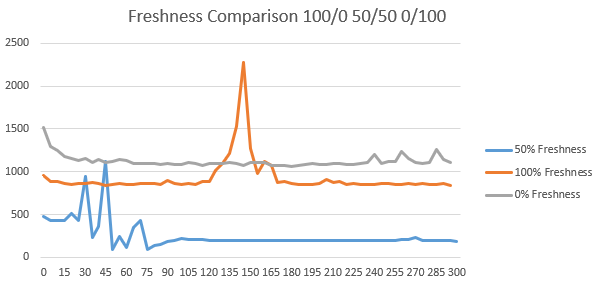
\includegraphics[width=0.7\textwidth]{Figures/fresh0.PNG}
    \caption{DQL only comparison, with varying degree of freshness}
    \label{fig:fresh0}
\end{figure}
These results generally show that the utilized freshness alone is already sufficient to provide better read results than if no freshness is used at all.
As before this is inherently caused by the targeted store of the query. While all queries without a freshness specification will directly contact a primary node,
hence needing to apply a lock. Although in general shared-locks can be easily applied for regular read-operations, they still need to be formally acquired impacting
the throughput. The most benefit can tehrefore be gained by combining the freshness with regular operations. As depicted above, these combinations provide by far 
the best results. Despite that regular reads still need to acquire a lock, these different query types will conseqeuntly also target different stores. 
This allows an efficient load distribution across the utilized stores, to harvest the benefits of a distributed environement.\\


Even with a mixed workload without freshness it is obvious that the store constellation does have an impact on the overall latency.
While regular queries (without freshness) will always target the primary placement, the selection which store to choose as a secondary
is crucial to provide better response times.\\


\begin{figure}[t] 
    \centering 
    \begin{tikzpicture}
        \begin{axis}[
            width  = 0.9*\textwidth,
            height = 7cm,
            x=120pt,
            major x tick style = transparent,
            ybar=.2cm,
            bar width=30pt,
            ymajorgrids = true,
            ylabel = {Avg. Response Time (ms)},
            xlabel = {Freshness Degree},
            symbolic x coords={0\%,100\%},
            xtick = data,
            scaled y ticks = false,
            enlarge x limits=0.40,
            ymin=0,
            ymax=4000,
            minor y tick num=4,
            major tick style={thick},
            legend style={
                    at={(1,1.05)},
                    anchor=south east,
                    column sep=1ex
            },
            legend cell align=left,
        ]
            \addplot[style={bblue,fill =bblue,mark=none}]
                coordinates {(0\%, 2504.659922) (100\%,3050 )};

            \addplot[style={rred,fill=rred,mark=none}]
                coordinates {(0\%, 2620) (100\%,2856.9465) };

            \legend{HSQLDB(Eager) - PostgreSQL(Lazy),
                PostgreSQL (Eager) - HSQLDB (Lazy) 
            }
        \end{axis}
    \end{tikzpicture}
    \caption{Mixed Workload HSQLDB vs. PostgreSQL}
    \label{fig:mixed}
\end{figure}

The illustration in \ref{fig:mixed}, therefore indicates the impact a store selection has on the overall throughput.
While regular operations perform better in the configuration targeting HSQLDB as the priamry node,
whereas queries with freshness target the secondary, which essentially flips the roles.
This is again caused by the target of the select statements. 
Since we are rather in a read-heavy environemnt the selection has quite the impact on the final result.
This again proves the point that the store selection will have a major impact.


%%%%%%%%%%%%%%%%%%%%%%%%%%%%%%%%%%%%%%%%%%%%%%%%%%%%%%%%%%%%%%%%%%
\subsubsection{Mixed Worklaod} 

Now with every building block evaluated independently, we will combine and assess them jointly using a mixed workload.


%%%%%%%%%%%%%%%%%%%%%%%%%%%%%%%%%%%%%%%%%
% Mixed with Freshness comparison
%%%%%%%%%%%%%%%%%%%%%%%%%%%%%%%%%%%%%%%%%

Based on the elementary comparison in Figure \ref{fig:write_decomposition} we have already established the impact on the capture-queue as well as the 
replication have on a single operation.

As mentioned in the implementation, depending on the current load on the system, we might observe contentions since the replication is done in parallel.
Furthremore we might even come across situations where an administrator will directly define a placement as \emph{INFINITELY OUTDATED} to not receive any more updates
and retain its current version.\\
For the next benchmark we therefore want to see how the workload behaves if the replicaton is done in parallel, if the replication distribution is suspeneded
and if the entire queue-capture is suspended.
This is again done using two HSQLDB stores, to reduce possible deviations across stores. 
Additionally this benchmark introduces freshness queries, to observe how it influences the overall response time even when there is no active replication. 
The freshness evaluation utilizes a freshness-index of $0.7$ to filter and identify possible candidates based on the number of received modifications.


\begin{figure}[t] 
    \centering 
    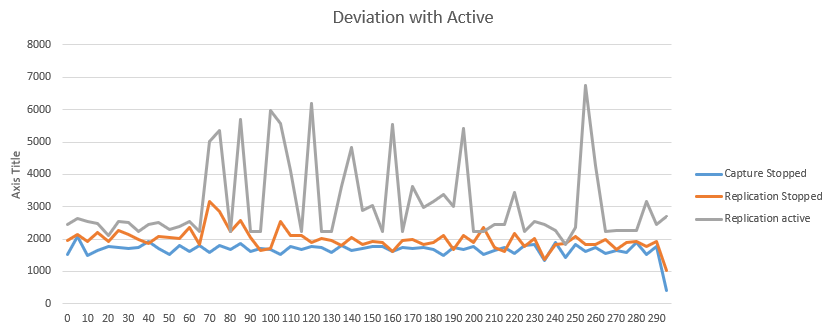
\includegraphics[width=0.7\textwidth]{Figures/deviation_with_active_que.PNG}
    \caption{Mixed Workload 60-40 with 100\% Freshness with relative read 1 minute }
    \label{fig:replication_impact}
\end{figure}

As provided by \ref{fig:replication_impact} we can again observe that the overal response time improves if there is no active replication running in the background.
Furthermore, the system performs best if it does not need to capture any changes at all, 
which essentially corresponds to the observations we have described in Figure \ref{fig:write_decomposition}.
Although this is rather a corner case, the replicaiton suspension on the other hand is more likely to occur and still provide good response times.\\

What is further interesting are the spikes on the active replication graph. While the graphs without replication and capture mechanisms are more narrow,
the active replication queue oscilates quite heavily, negativiely impacting the average response time.\\
Further, we observe that these spikes start occuring after roughly one minute.
Since we used a modification deviation for our freshness specification, the system is able to quickly identify suitable placements in the beginning of the benchmark.
However, after some time the versions start deviating quite heavily from its eager version.
Since the updates are only propagated operation-wise, the replications cannot catch up with the primary operations anymore.
Hence the system is not able to fulfil the tolerated freshness-level and
causes the algorithm to fall back to its primary placement, again investing additional time to combine and select a suitable combination of placements.\\




%%%%%%%%%%%%%%%%%%%%%%%%%%%%%%%%%%%%%%%%%
% Partition
%%%%%%%%%%%%%%%%%%%%%%%%%%%%%%%%%%%%%%%%%
\subsubsection{Partitioning} 

Our freshness and replication implementation essentially revolves around the handling of individual partition placements.
However, so far all tests only really considered unpartitioned entites to visualize basic differences. 

\begin{figure}[t] 
    \centering 
    \begin{tikzpicture}
    \begin{axis}[
        width  = 0.8*\textwidth,
        height=6cm,
        x=80pt,
        major x tick style = transparent,
        ybar=.2cm,
        bar width=25pt,
        ymajorgrids = true,
        ylabel = {Avg. Response Time (ms)},
        xlabel = {Partition Constellations},
        symbolic x coords={1},
        xtick = data,
        xticklabels={},
        scaled y ticks = false,
        enlarge x limits=0.40,
        ymin=0,
        ymax=3000,
        minor y tick num=4,
        major tick style={thick},
        legend style={
                    at={(1,1.05)},
                    anchor=south east,
                    column sep=1ex
            },
        legend cell align=left,
    ]
        \addplot[style={bblue,fill =bblue,mark=none}]
            coordinates {(1, 444.19055)};

        \addplot[style={rred,fill=rred,mark=none}]
            coordinates {(1, 364)};

        \addplot[style={ggreen,fill =ggreen,mark=none}]
            coordinates {(1, 2395)};

        \legend{ 
            5 Stores - 4 Partitions,
            2 Stores - 4 Partitions,
            2 Stores - Unpartitioned
            }
    \end{axis}
\end{tikzpicture}
    \caption{Impact of Partitioning on Freshness across Lazy Replicated Stores.}
    \label{fig:partition_result}
\end{figure}

Accompanied with the introduced locking changes described in Figure \ref{fig:lock_comp} we will compare the mixed workload in 
a partitioned environement. For one we partition the table into four horizontal partitions. 
For one scenario we place all partitions on the eager node and then each partition respectiviely on four lazy replicated stores.
The second scenario will place all four partitions across two stores, where exactly one is eagerly and the other lazily replicated. 
These two variations are ultimately compared against an entire unpartitioned setup across two stores which is visualized in \ref{fig:partition_result}.


Analogously to the results obtained from the locking mechanism bechmarks, consequently
these results indicate, that we achieve the best performance
if we indeed partition the entity and place all partitions on each entity across both stores. Therefore the system will have the most possible 
flexibility in locking and acessing the individual data fragements. Although 
it is still a comparably good alternative comapred to teh unpartitioned configuration.\\


%%%%%%%%%%%%%%%%%%%%%%%%%

Concluding with the evaluations as illustrated with the last examples and benchmarks, the results of using freshness, inherently differs by means of the utilized workload.
Figure \ref{fig:workload_comp} therefore ultimately presents the impact of the workload on freshness-aware data management in general. 

\begin{figure}[t] 
    \centering 
    \begin{tikzpicture}
        \begin{axis}[
            width  = 0.9*\textwidth,
            height = 7cm,
            ymajorgrids = true,
            ylabel = {Throughput (requests/s)},
            xlabel = {Workload (R/W)},
            symbolic x coords={100,(80/20),(60/40),(50/50),(40/60),(20/80),(0/100)},
            xtick = data,
            scaled y ticks = false,
            enlarge x limits=0.1,
            minor y tick num=1,
            ymin=0,
            ymax=60,
            major tick style={very thick},
            legend pos=outer north east,
            legend cell align=left,
            smooth
        ]
            \addplot[style={bblue,mark=*}]
                coordinates {
                    (100, 54.7044553) 
                    ((80/20),16) 
                    ((60/40),10.4) 
                    ((50/50),12.52163117) 
                    ((40/60), 15.56761) 
                    ((20/80),16.99402276) 
                    ((0/100),19.05664)
                    };

        \end{axis}
    \end{tikzpicture}
    \caption{Worklaod Comparison of Freshness Related Queries}
    \label{fig:workload_comp}
\end{figure}

As we have identified before the most extreme cases like read-only and write-only workloads achieve the best results,
since there are no negativiely impacting concurrent operations.
However, because these are not common workloads the next best operation is considered to be a write-heavy worklaod focussing.
This essentially mimics a highly transactional workload using the reads mainly for analytical purposes.


This shows that freshness-aware data management can indeed allow to improve mixed workloads during write-heavy situations.




%%%%%%%%%%%%%%%%%%%%%%%%%%%%%%%%%%%%%%%%%%%%%%%%%%%%%%%%%%%%%%%%%%
%%%%%%%%%%%%%%%%%%%%%%%%%%%%%%%%%%%%%%%%%%%%%%%%%%%%%%%%%%%%%%%%%%
%%%%%%%%%%%%%%%%%%%%%%%%%%%%%%%%%%%%%%%%%%%%%%%%%%%%%%%%%%%%%%%%%%





\section{Discussion}
\label{sec:discussion}

The results generally show that although the replication will slightly mitigate the overall performance of the system, it still is able to correctly fulfil the 
requirements without largely interfering with the underlying systems. 
Despite that the operation-wise execution will gradually progress each state the capture-queue inherently impacts the preformance.\\

However, the compound results shows that freshness related queries are indeed suitable candidates when not focusing on a pure mixed-workload with equal amounts of read and write-operations.

Although, the freshness queries provided promissing results, they still suffered from a rather static freshness specification. 
Therefore it would make sense to extend and adapt the utilized benchmarks to adaptively adjust the degree of freshness during runtime
as needed and still providing reproducible results.



%%%%%%%%%%%%%%%%%%%%%%%%%%%%%%%%%%%%%%%%%%%%%%%%%%%%%%%%%%%%%%%%%%




